%******************************** Fifth Chapter *******************************************************
%******************************************************************************************************

\externaldocument{{../Chapter1/chapter1}}
\externaldocument{{../Chapter2/chapter2}}
\externaldocument{{../Chapter3/chapter3}}
\externaldocument{{../Chapter4/chapter4}}
\externaldocument{{../Chapter6/chapter6}}
\externaldocument{{../Chapter7/chapter7}}
\externaldocument{{../Appendix1/appendix1}}
\externaldocument{{../Appendix2/appendix2}}
\externaldocument{{../Appendix3/appendix3}}
\externaldocument{{../Appendix4/appendix4}}
\externaldocument{{../Appendix5/appendix5}}
\externaldocument{{../Appendix6/appendix6}}
\externaldocument{{../Appendix7/appendix7}}
\chapter{Future Work}
\label{future}

% **************************** Define Graphics Path **************************
\graphicspath{{Chapter5/Figs/}}

This work has served as a proof of concept upon which future developers would be able to build to vastly improve the behaviours of the stock ArduPlane autopilot. Although this work has not provided a complete solution to the problem, it has provided a basis from which a more complete and robust solution could be implemented. This project has opened up a number of avenues for improvement and extension, and this chapter shall be suggesting and discussing a few of them.  All of the proposals in this section would make suitable candidates for the next body of work to be completed, partly as none of them rely on any other proposal to be beneficial to the overall project. 

The proposals that shall be discussed are

\begin{enumerate}
	\item Incorporation of path planning solution into mission planning software
	\item Improving tolerances in path planning solution
	\item Alternate techniques for commanding UAV navigation along Dubins paths
	\item Planning Paths Onboard the UAV
	\item Improving the handling of wind gusts
	\item Extending Dubins path turning to work in 3D space
\end{enumerate}


%******************************************************************************************************
%******************************************************************************************************
\section{Proposal 1: Incorporation Into Mission Planning Software}
\label{future:missionplanner}
This proposal could be completed at any time, either now or once a more complete solution is developed, but mainly focuses on usability as opposed to functionality. 

\subsection{Proposal 1: Justification} 
\label{future:missionplannerreason}
In order to make the planning process simpler for the user, incorporating the path planning application into the mission planning software is a must. Both MissionPlanner and APM Planner 2, as discussed in Section \ref{intro:planner}, are open source applications. This means it would be quite straight forward to incorporate our path planning software into each program, but would require work on both codebases. By integrating our work into the mission planning software, we would be able to specify new types of waypoint to signify the start and end points of each imaging path, and the planning software could calculate the desired Dubins path between the two, when provided with a wind input. This would also enable us to automatically generate the turn commands issued to the UAV in the mission plan, meaning no user intervention would be required to edit them. 

\subsection{Proposal 1: Plan} 
\label{future:missionplannerplan}
The first step would be to download and analyse the operation of the two path planning applications. Following this it would be necessary to either re-write our planning application, or simply call it from within the planning software to return the results. This should be straightforward, however as the author has not been working with either of these codebases, suggesting a time estimate for this work would not be wise. 

After implementing the changes, we could issue a pull request for the repositories on GitHub and our changes may be included into the officially released versions.

\subsection{Proposal 1: Summary}
\label{future:missionplannersummary}
This change would be both straightforward to implement and hugely beneficial to the average user. It would massively simplify adding our new turn techniques into a mission and remove the need for tinkering and editing of mission plans.

As this project has been essentially a proof of concept and was never intended to be incorporated into official ArduPilot products, it has not been necessary to do this as part of the project. If it were included as part of this project, it would have been very useful for speeding up the testing process, as currently it is necessary to edit the mission plans manually. 

%******************************************************************************************************
%******************************************************************************************************
\section{Proposal 2: Improving Tolerances at the Planning Stage} 
\label{future:tolerance}
This proposal aims to improve performance of the system as a whole, enabling the UAV to recover from unfavourable wind conditions.

\subsection{Proposal 2: Justification}
\label{future:tolerancereason}
Whilst the UAV is performing one of our newly implemented turns, it could be unexpectedly blown off course by a gust of wind. In its current form, the new turning system banks the UAV at its maximum permitted bank angle to completed left and right turning segments. If we imagine the UAV performing a right hand turn segment, and being blown off its course to the left; it is unable to command a greater bank angle and as such will never return to the original turning path. If we are aware of the wind speed and the likelihood of gusts at the planning stage, we can instead plan a route using a more shallow bank angle to give us some leeway in the bank commands. This means that should we be blown off course, we can command more of a bank to enable us to return to the original intended path, followed by reducing the bank angle to its original value. 

Adding this tolerance in at the planning stage would ensure improved performance in gusty conditions, and would reduce the risk of missing the start point of our imaging paths with the correct orientation.  

\subsection{Proposal 2: Plan} 
\label{future:toleranceplan}
The new planning algorithm would need to take into account wind gusts, but in their very nature these are hard to predict. One solution to this would be to plan all routes with very conservative turning radius, requiring smaller bank and roll angles. Another alternative would be to base our bank and roll angles off the magnitude of a wind average; if the average wind speed over a period of time during the planning stage is low (such as 5 metres per second) we can safely use greater roll and bank angles, and as such reduce our turning radius. 

Neither of these proposed solutions are particularly pre-emptive of the behaviour of the wind, but would both enable us to accurately track a turning path regardless of gusts. A final solution would be to use a weather mapping service for the area which provides a range of wind speeds we can expect. There are a number of online meterological services that can provide an average wind speed with a predicted speed that gusts may reach. Using the ratio of expected gusts to current wind speed (with allowances either side for inaccurate readings) we can derive a suitable roll and bank limit for our flight.

Once we have calculated the suitable roll angle values, they could be passed in with the MAVLink commands to be set during the flight. The current implementation simply uses the UAV's maximum roll angle, instead we would pass another value in one of the spare parameter fields to set a specific roll angle. We would also need to implement a system to detect gusts and correct tracking after the fact, for this we would also need to implement Proposal 5 in Section \ref{future:gusts}. Other than this very little would need to be changed, as we would be able to calculate our minimum turning radius from our desired speed and roll angles, and then use the rest of the system as is. 

\subsection{Proposal 2: Summary} 
\label{future:tolerancesummary}
This proposal would provide a much greater level of reliability to our system to help ensure that environmental factors don't cause the UAV to miss the start of imaging paths. The most difficult aspect would be gathering accurate information about the behaviour of the wind, a very difficult set of variables to record. The most straightforward option would be to simply use very conservative roll limits combined with the features of Proposal 5. This would still improve reliability but we would not be making the absolute most of our battery life by maximimising performance. Like many things with this kind of work, it is a compromise between performance and reliability that needs to be considered, alongside determining how this sort of solution would work for a large range of UAVs with very different flight characteristics. 

%******************************************************************************************************
%******************************************************************************************************
\section{Proposal 3: Alternate Techniques for Dubins Path Navigation} 
\label{future:alternatedubins}
In its current state, we simply command the UAV to fly a Dubins path by specifying a time value and whether to turn left, right, or fly straight. Whilst this works, there are alternatives which may yield better results through improved reliability. Once again this is a performance improvement, focussing on reliability, but should not in theory improve performance in terms of battery usage.

\subsection{Proposal 3: Justification}
\label{future:alternatedubinsreason}
One of the alternatives considered throughout the planning phase was to utilise the already existing waypoint following capabilities of ArduPlane to perform a Dubins path turn. Fig. \ref{fig:waypointdubins} shows how this would work. We would place our waypoints at the points at which we transition between segments of the Dubins path in order to perform the turns. One caveat of this would be that we would need to update these positions very frequently to account for the effects of wind, which would need to be carefully integrated with the navigation system to ensure we were commanding the UAV to fly to the correct place. For this project it was decided this approach was too risky, as the need to regularly the waypoint location could cause issues, not least because waypoint locations are define by GPS locations, and calculations involving GPS locations may be too intricate and not quick enough to deliver suitable computational speed. Alternatively, it would be possible to define the waypoint location as a position relative to the UAV at the start of the Dubins path turn, but again the computational requirements would be high and could produce timing issues such as race conditions. 

\begin{figure}[htbp!] 
\centering    
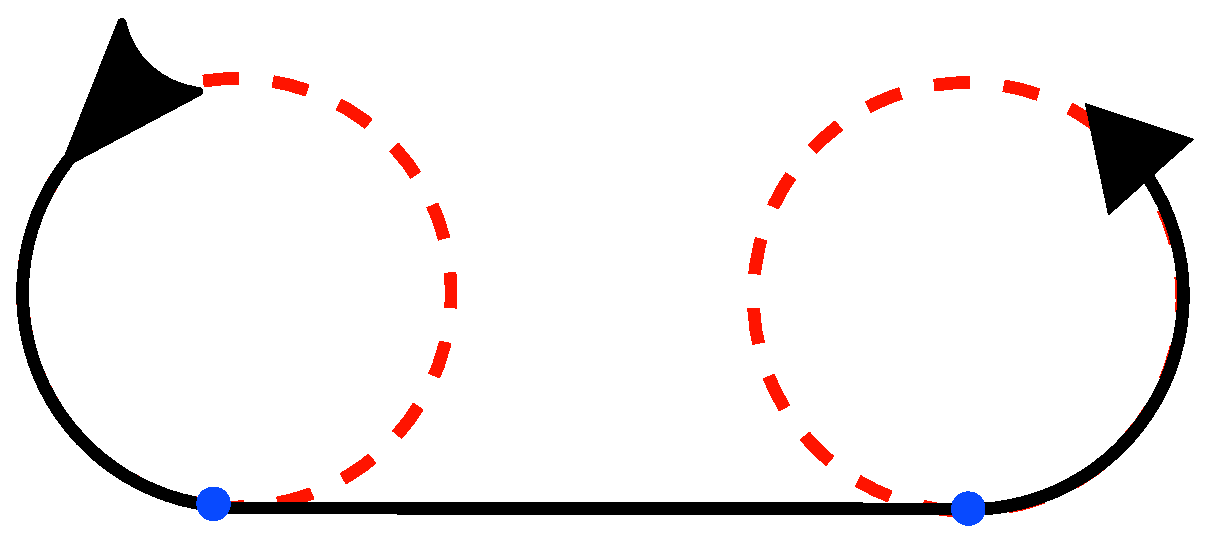
\includegraphics[width=0.5\textwidth]{WaypointDubins}
\caption[Commanding a Dubins path turn using waypoint navigation]{Using the existing waypoint navigation system to command a Dubins path turn}
\label{fig:waypointdubins}
\end{figure} 

Another alternative that was considered was to leverage the loitering capabilities of ArduPlane to command left and right hand turns. An example of how this would work can be seen in \ref{fig:loiterdubins}, where we place a waypoint at the centre of the circle formed by the extended arc we intend the UAV to travel . The issue seen with this would be that we would have to ensure that the UAV was in exactly the correct place when commanded to start the loiter segment, or else we would introduce irregularities into the path that would extend the length of the path and potentially throw off the entire process and cause the UAV to miss the virtual target intercept. Also, we would need to update the waypoints in much the same way as for the solution proposed in Fig. \ref{fig:waypointdubins}.

\begin{figure}[htbp!] 
\centering    
\includegraphics[width=0.5\textwidth]{LoiterDubins}
\caption[Commanding a Dubins path turn using loiter navigation]{Using the existing loiter navigation system to command a Dubins path turn}
\label{fig:loiterdubins}
\end{figure} 

Both of these solutions were considered too risky to attempt for this project, but could potentially provide excellent results if implemented correctly. By using the pre-existing navigation techniques we would by default be providing a method to correct cross-track error and as such more accurately track the desired path. However, as the path itself would be being regularly updated to counter the effects of wind, it is hard to know exactly how the UAV would behave. Deeper understanding of the ArduPlane navigation code would be required, or failing that just trying to implement this would tell us how they would perform.  

\subsection{Proposal 3: Plan} 
\label{future:alternatedubinsplan}

Both of these solutions would require changes to the default navigation system, both for loitering and for straight line following. The need to update the waypoint location could result in paths that are not smooth, negatively impacting battery usage and requiring frequent control inputs to the UAV, further increasing the risk of generating cross-track error. An alternative to this would be to find some way to define the waypoints as air relative locations, removing the need to update their position. This could be done if we have accurate values for the wind speed on board the UAV by calculating our position relative to the air using the GPS location and the wind values. 

Regardless of the approach used, this would be a very large undertaking, one which was considered too large and too risky for this project. Implementation and simulation would be the only true test of its performance however, making it hard to speculate on its benefits.

\subsection{Proposal 3: Summary} 
\label{future:alternatedubinssummary}

This proposal would be difficult to implement, as it is hard to know the exact location of the UAV relative to the air. Airspeed sensors would need to be combined with knowledge of the environmental factors to provide accurate location data, which could then be used as part of a navigation system. Also, this would require airspeed sensors on the UAV which would be additional to the minimum requirements to fly a UAV using ArduPlane.

We would also need to ensure that any paths generated from a moving waypoint would either be generated as smooth lines, or have them smoothed via some mathematical process, some form of spline function perhaps.

%******************************************************************************************************
%******************************************************************************************************
\section{Proposal 4: Planning Paths Onboard the UAV} 
\label{future:onboard}

Currently our system plans our new turns entirely on the ground. If we are able to calculate our paths on the UAV, it would allow us to better handle disturbances by wind.

\subsection{Proposal 4: Justification}
\label{future:onboardreason}

When we plan our paths we need to know the orientation of the UAV when starting the turn, as well as when we finish it. If we imagine a scenario in which we are reaching the end point of an imaging path and we need to start our turn, it is possible that a gust of wind has blown us off course or altered our orientation. By calculating the path when we are about to reach the start point of the turn, we can instead use accurate values for our orienation and as such plan a more suitable path. 

Further to this, if the wind speed increases or changes direction, we would be able to plan a new route to handle these changes, resulting in better alignment with the imaging path and providing higher quality aerial photographs. 

\subsection{Proposal 4: Plan} 
\label{future:onboardplan}

Our first consideration for this work would be whether the hardware currently available would be suitable. As discussed in Chapter 1, the APM boards do not have the storage capacity for even the latest stock versions of ArduPlane, so would definitely not be able to accommodate an additional feature such as this. The Pixhawk board may be able to, but this would need to be investigated beforehand. Another consideration is processing power; the current algorithm is a form of search algorithm, and depending on the input parameters may take a little while. The processors on both the Pixhawk and the APM are not massively powerful, so processing time would need to be a consideration. 

One solution to this would be to introduce some dedicated hardwre to handle the task. We could add an additional processor that could be connected up to the controller board and sensors which would then be solely responsible for calculating Dubins paths for the autopilot to use. Although this would introduce additional costs and weight to be carried, it would ensure that calculating these paths would not slow down the navigation systems or hog the processing power of the controller board.

With regards to the software itself, if we were to provide additional hardware, the only thing we would need to do would be to port it to the new device and configure it to take its inputs from the autopilot. If we were integrating it to ArduPlane, the process would be even easier, simply passing variables from within the autopilot system itself without the need to enable communication protocols or sensor connections. 

It may prove necessary to define a new processing algorithm to find a suitable Dubins path. Currently, we attempt to solve each of the Dubins path types for each set of inputs and then see if they meet our virtual target intercept criterion. If there was some way to simplify this process so that we were not assessing all 6 path types for each iteration of the algorithm, it would reduce the time taken to find a solution, and thus reduce our processing requirements. Currently the author is unaware of any such solution, so further investigation would be required.

\subsection{Proposal 4: Summary} 
\label{future:onboardsummary}

This is another proposal that could generate real performance improvements, and take the current solution one step closer to a system that would be suitable for operation in any wind condition. Calculating the paths on the UAV would introduce additional demand on processing, however the performance improvements we could expect may be worth any hardware investments to some users. One of the major drawbacks of the current system is its inability to handle the effects of wind gusts; this proposal would allow just that. 

%******************************************************************************************************
%******************************************************************************************************
\section{Proposal 5: Improving Handling of Gusts of Wind} 
\label{future:gusts}

As briefly touched upon in Proposal 2 (section \ref{future:tolerance}), this proposal aims at improving the systems ability to correct for perturbations due to gusts of wind. Again this is an improvement to performance, in particular to improve system reliability. 

\subsection{Proposal 5: Justification}
\label{future:gustsreason}

The ability to correct cross-track error generated by gusts of wind is important in any UAV navigation system, as gusts are unpredictable in both magnitude and duration. If we are able to correct disturbances from gusts during our new type of turn, we can ensure that we are correctly aligning the UAV with the imaging path as desired. This can help us to both improve battery usage by ensuring we take the most suitable path, whilst also helping to ensure high quality aerial images are captured by guaranteeing the UAV aligns with the next imaging path. 

The navigation system currently in use in ArduPilot has the ability to correct disturbances and reduce cross-track error, but the current implementation of our turning mechanism does not. 

\subsection{Proposal 5: Plan} 
\label{future:gustsplan}

In order to implement this proposal we would need a way to better define the path segments that the UAV is following. As it currently works, the UAV has no knowledge of the overall shape of the Dubins path we are commanding it to follow, only which direction to turn (L, R, or S) and for how long. In this respect, the work proposed in Proposal 3 (Section \ref{future:alternatedubins}) would solve this issue. 

Another solution would be to calculate the ground relative path for the UAV to follow, and to use a similar navigation system as is currently in place to follow it. This would require considerable changes to the current path planning software, as it would need to introduce curved paths that are calculated as a feature of wind. Our work so far provides a means for us to calculate these routes, but no way for us to define it within the mission plan. Currently, the mission plan for an ArduPlane mission is not capable of defining curved paths, except for as loiter paths, so work would need to be done in this regard. The navigation system in place currently calculates cross-track error by comparing the GPS position of the UAV with the vector between the previous waypoint and the next waypoint, which is of course represented by a straight line. In order for the UAV to recognise curved paths, we would need information included in the mission plan to define these curves to enable us to calculate and correct cross-track error. 

As mentioned, the completed work on this project provides us with a method for plotting a complex curved path in the form of a matrix of co-ordinates. Although it is not complicated to collect this data, it would be difficult (if not impossible) to load it all onto the UAV. A potential solution would be to limit the number of values in order to create a series of very short lines connecting a large number of waypoints, which when flown would essentially form a curve. This may be possible on the Pixhawk board as it is capable of storing a large number of waypoints, but would limit the maximum size of any mission implementing this technique. Further research into the viability of this work would need to be conducted.

\subsection{Proposal 5: Summary} 
\label{future:gustssummary}

For us to be able to correct cross-track error we need a new method for defining our Dubins paths. This would be a very large undertaking but could result in massive improvements in performance, stability, and resilience to environmental factors. The work completed in this project would provide a great starting point for this work, but would require a complete redesign of all of the changes made to ArduPlane for it to work.

%******************************************************************************************************
%******************************************************************************************************
\section{Proposal 6: Extending Path Planning to Work in 3D} 
\label{future:3d}

This final proposal is aimed at extending the range of applications for which we can use our new Dubins path turning mechanism. It would not improve performance, but instead add additional functionality that may prove useful in a number of photogrammetry scenarios.

\subsection{Proposal 6: Justification}
\label{future:3dreason}

In its current form, our system enables improved turning for aligning with imaging paths in only the 2D plane. If we wanted to fly at different altitudes for adjacent imaging paths we would need to add in additional waypoints to first alter our altitude, and then align with the next imaging path. If we were able to incorporate an altitude change into our current system, we could improve battery usage for any aerial photography usage requiring altitude changes. This would be particularly useful when surveying any area which displays large changes in elevation such as steep hillsides, mountains, or glaciers. By incorporating this change we would be able to keep a consistent relationship between a given area on the ground and the number of pixels that show that area. This means that once captured, the images would be able to be stitched together and display consistent resolution, removing the need to edit our collected images.

\subsection{Proposal 6: Plan} 
\label{future:3dplan}

Research documented in \cite{beard2013implementing}, \cite{hota2010optimal}, and \cite{lin2014path} show that this proposal is not only possible, it is effective too. Using the current navigation system available in ArduPlane, it would not be too much extra work to include our third axis of movement, whereby controlling for pitch changes could be carried out at the same time we alter roll and yaw. As with the current system, we would need to include allowances for disturbances and error due to wind and gusts, but in essence the navigation system would be relatively unchanged. The current waypoint navigation system accounts for changes in altitude, so if it was extended as proposed in Proposal 5, it would also be able to correct errors in $z$ axis. 
%TODO polish off this section

\subsection{Proposal 6: Summary} 
\label{future:3dsummary}

As with all of the proposals so far, this of course an element of uncertainty in regards to the effectiveness of this change. Whilst it would of course be a very useful change, if someone were to extend on this work of this project, this would not be the highest priority task moving forward. The actual changes to the path planning would not need to be too vast, we currently have three new commands relating to this project; turn left, turn right, and go straight. Adding 3D Dubins path turns would require us to specify a pitch angle too, however this could simply be included in the existing MAVLink commands and used when carrying out the regular commands. All in all this feature would not be too much extra work and would definitely improve the usefulness of this project, particularly as using UAVs for mapping unforgiving terrain is an attractive prospect and this proposal would help us to do so.

%******************************************************************************************************
%******************************************************************************************************
